\documentclass[12pt,a4paper,draft]{article}
\usepackage[utf8]{inputenc}
\usepackage[english]{babel}
\usepackage{amsmath}
\usepackage{amsfonts}
%\usepackage{amssymb}
\usepackage[left=2cm,right=2cm,top=2cm,bottom=2cm]{geometry}
\author{Adrian Bach}
\title{Assessing visual representation of uncertainty in conservation policy makers-directed documents.}

\begin{document}
\maketitle

\tableofcontents

\section{Context \& Purpose}

Workshop in NINA.
Preliminary title "Communicating uncertainty from resource management models".
Group 2: visual representation of uncertainty and users perception.
Assessing the way uncertainty about scientific data (measures and models results) is currently represented in documents directed to conservation policy-makers.
Kinkeldey et al. (2013) reviewed papers about uncertainty representation in scientific papers, identifying five different levels of dichotomies.
\begin{itemize}
\item Explicit (uncertainty obtained from the data) / Implicit (displaying all the possibilities)
\item Extrinsic (new objects to represent uncertainty, \textit{e.g.} skewers, glyphs, intervals) / Intrinsic (altering the data visuals, \textit{e.g.} play on colors and shapes)
\item Visually integral (make sense only combined with the data) / Visually separable (still make sense when  separated from the data)
\item Coincident (represented in the same place as the data) / Adjacent (represented in another box than the data one's)
\item Static (inanimate figure) / Dynamic (interactive figure)
\end{itemize}
Used these categories to characterize uncertainty representation in figures from a significant number of policy documents from different conservation organisations.
In order to produce a bar plot of the frequency of use of each combination of representation.
Beside giving a good idea of the current habits for uncertainty representation in conservation, it will also be interesting to compare the results with the best practice that will come out of the paper, and also target more accurately the areas of possible improvement.

\section{Methods}

Search for documents with internet browser.
Currently 24 figures reviewed from documents produced by the following organisations: European Environmental Council (EEA), Scottish National Heritage (SNH), Joint Nature Conservation Committee (JNCC), Australia's Convention on Biological Diversity (CBD).
For each figure in which uncertainty representation was relevant, gathered in a csv file first the organisation, the focal natural feature, the year of production in text, for the first part.
Then, attributed a binary code (respectively 0 / 1 in the following categories) to if uncertainty representation was absent / present, explicit / implicit, extrinsic / intrinsic, visually integral / separable, coincident / adjacent, static / dynamic.
Using R, combined these information in a single binary number (\textit{e.g.} a present representation of uncertainty being explicit, intrinsic, visually separable, coincident, and static would be 100100).
That way, each specific combination had a unique binary code, which I converted into a unique decimal number for convenience (same example, 100100 would be a 9).
With the pivot table tool on excel, created a stacked bars plot displaying the counts of each combination, with a color code for the type of figure.
Counts might be changed to actual frequency when increasing the number of reviewed figures.

\section{Preliminary results}

\begin{figure}
\centering
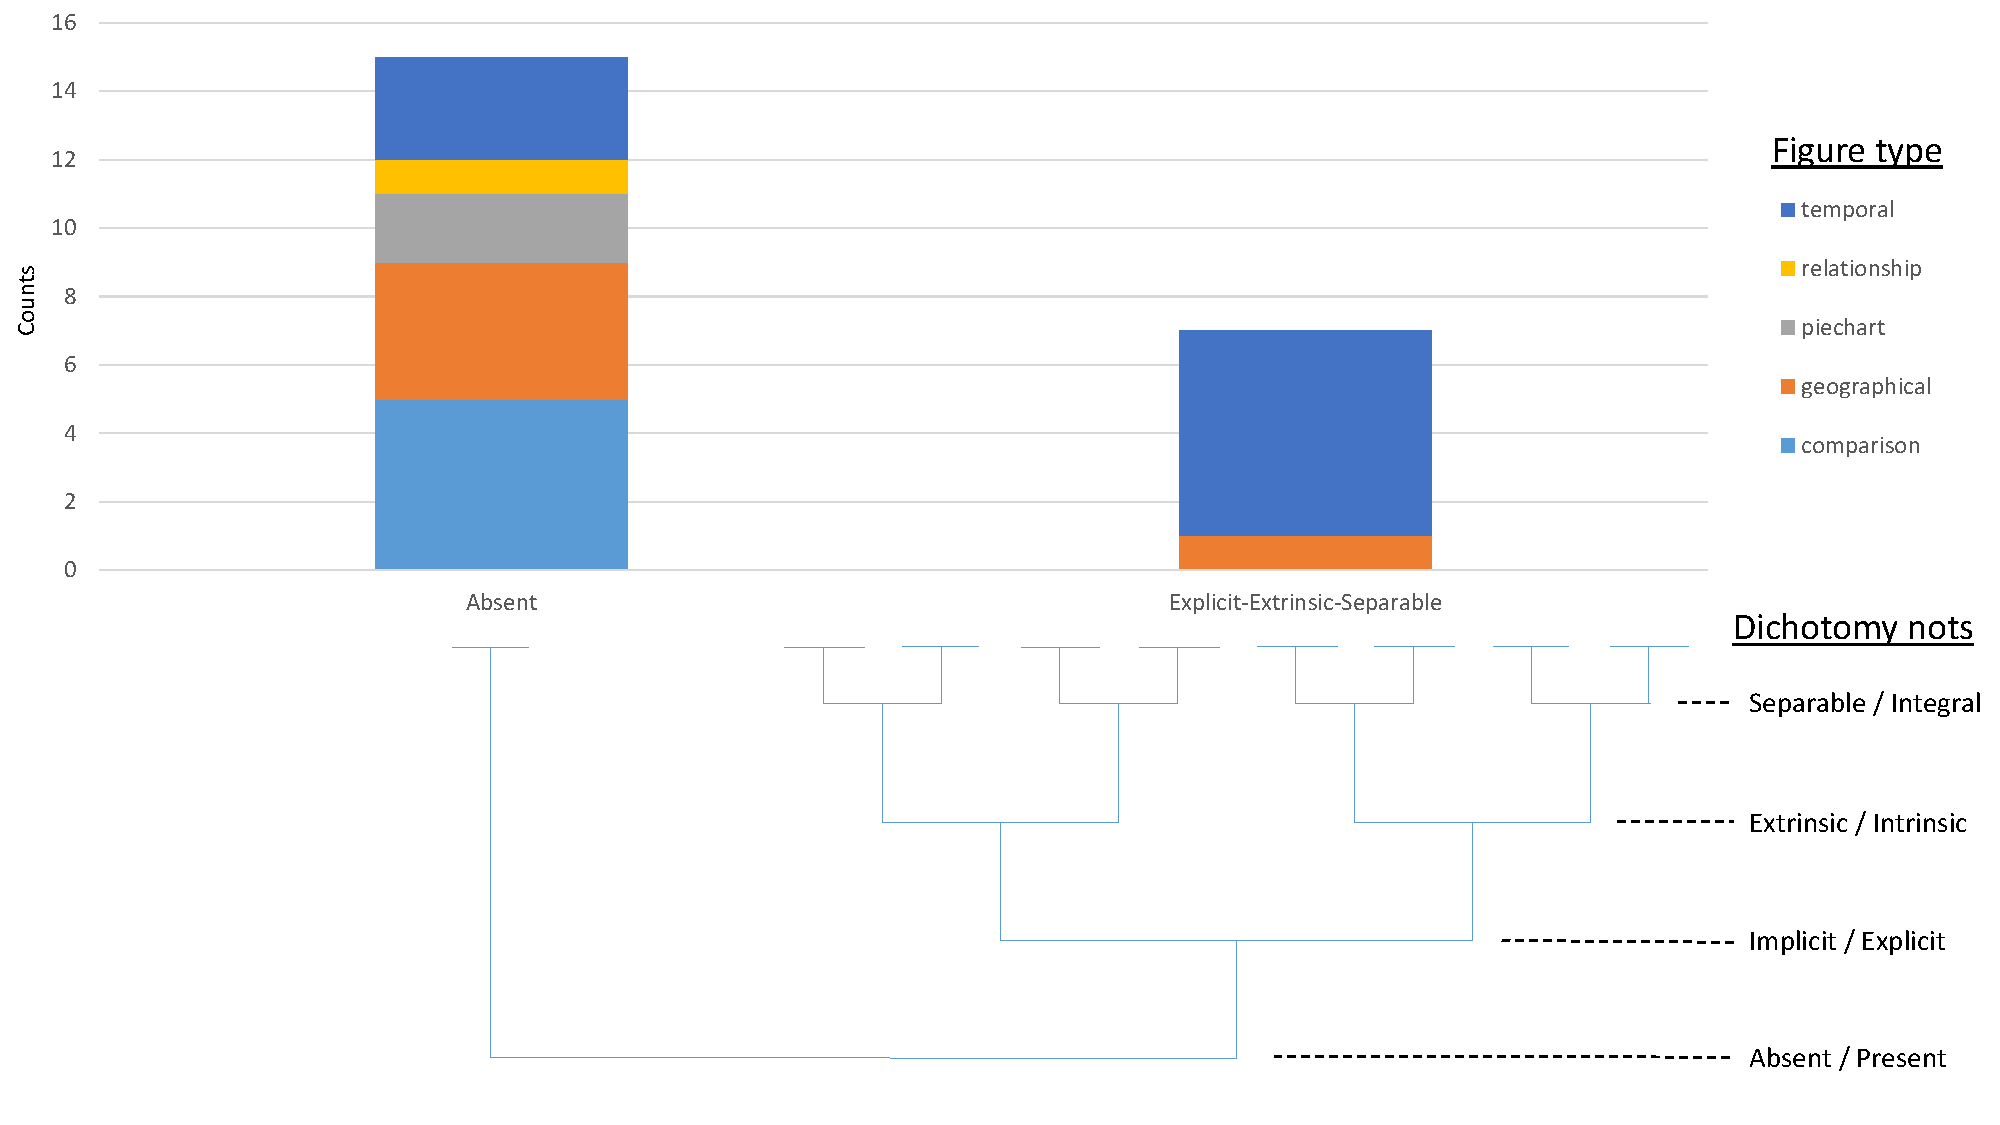
\includegraphics[scale=0.25]{uncertainty_representation_review_fig.pdf}
\caption{Preliminary representation of the review results.}
\label{prelifig}
\end{figure}

Uncertainty was not represented in 70\% (N = 24) of the reviewed figures.
When represented, only the explicit-extrinsic-visually separable combination has come out for now.
No adjacent representation, or dynamic figure has come out yet.
As suggested in Kinkeldey et al. (2013), it seems unlikely that an extrinsic representation of uncertainty would not as well be visually separable from the data.
The majority of the figure in which uncertainty was represented were temporal evolution figures, in the form of standard deviation or confidence intervals (6 out of 7, or 85\%).
Unexpectedly, uncertainty was not represented in any of the comparison figures, for which skewers are common practice in science.
In this sample, uncertainty was never represented in pie charts (for which intrinsic representation would be suitable?).



\end{document}